\SourcePage{GELFAND-P000451}{72}
\sout{\ldots}\quad with condition $1)$ $\psi(F^p,F^{n-p})=0$.
\Incomplete{GELFAND-P000451}{initial-cancel}{The short cancelled sign before “with” is undeciphered.}
\end{GelfandAdjacentEvidence}
\begin{GelfandAdjacentEvidence}{GELFAND-P000451}{2}

\Unclear{GELFAND-P000451}{orthogonality-exponent}{The first formula clearly reads $n-p$. The next formula separately reads $n-p+1$.}
\end{GelfandAdjacentEvidence}
\begin{GelfandAdjacentEvidence}{GELFAND-P000451}{3}


This is an algebraic subs. $\bar D$.

$\psi$ either symm. or skew-symmetric \uuline{(def)}.

\[
2)\quad F^p\oplus\bar F^{n-p+1}\cong H_{\mathbb C}
\]
\Unclear{GELFAND-P000451}{complement-sign}{The sign before $H_{\mathbb C}$ has a wave above two horizontal strokes. A slanted mark joins the lower strokes. The reading $\cong$ is provisional. The letter $H$ is heavily retraced.}
\end{GelfandAdjacentEvidence}
\begin{GelfandAdjacentEvidence}{GELFAND-P000451}{4}

\[
H_{\mathbb Z}\subset H_{\mathbb R}\subset H_{\mathbb C}
\qquad\mbox{\uuline{also given}}
\]

The nondeg. flag determ. the grading and the Weil autom.
\[
H^{p,n-p}=F^p\cap\bar F^{n-p}
\]
Weil autom.:
\[
C\xi=i^{2p-n}\xi\quad\text{when }\xi\in H^{p,n-p}
\]
These conds. pick out in $\bar D$ the open subs. $D$.

\sout{\ldots}\qquad Another condition:\quad $\psi(x,C\bar x)>0$ when $x\ne0$.
\Incomplete{GELFAND-P000451}{condition-cancel}{Several horizontal strokes cover the earlier writing before “Another condition”. The ending has a loop and a stop. The text is unresolved.}
\end{GelfandAdjacentEvidence}
\begin{GelfandAdjacentEvidence}{GELFAND-P000451}{5}


Define on $D$ the structure of a homog. sp..

$G$ — group of all real transf. of $H_{\mathbb R}$, preserv. $\psi$
\[
\bigl(\psi(gx,gy)=\psi(x,y)\bigr).
\]
\Unclear{GELFAND-P000451}{group-equation}{The left outer parenthesis is heavily retraced. Two round closing parentheses are distinguishable on the right.}
\end{GelfandAdjacentEvidence}
\begin{GelfandAdjacentEvidence}{GELFAND-P000451}{6}


\uwave{Then \mbox{$G$} acts on \mbox{$D$}}

\SourceFigure{GELFAND-P000451}{theorem-insert}{Before $G$ is a short inscription provisionally read as “яв.” (“expl.”) and a heavily retraced sign. A $1$ is inserted in the loop above it. The beginning of the line provisionally reads $1)$.
\par\smallskip\centering\color{black}
\begingroup\color{black}\GelfandFitDiagram{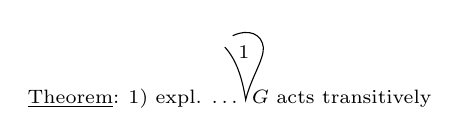
\begin{tikzpicture}[x=1mm,y=1mm,every node/.style={anchor=base west,inner sep=0pt,font=\scriptsize}]
\node (theorem) at (0,4) {\underline{Theorem}:};
\node (old) at ([xshift=1mm]theorem.base east) {$1)$ expl. \sout{\ldots}};
\node (g) at ([xshift=1.2mm]old.base east) {$G$ acts transitively};
\node at ([xshift=-1.7mm,yshift=5.7mm]g.base west) {$1$};
\coordinate (tail) at ([xshift=-.7mm,yshift=.4mm]g.base west);
\draw ([xshift=-3.35mm,yshift=7.1mm]g.base west)
  .. controls ([xshift=-1.95mm,yshift=5.6mm]g.base west) and
              ([xshift=-1.15mm,yshift=3.3mm]g.base west) .. (tail)
  .. controls ([xshift=-.05mm,yshift=3.15mm]g.base west) and
              ([xshift=1.6mm,yshift=5.45mm]g.base west) ..
              ([xshift=1.55mm,yshift=7.05mm]g.base west)
  .. controls ([xshift=1.35mm,yshift=8.75mm]g.base west) and
              ([xshift=-.25mm,yshift=9.5mm]g.base west) ..
              ([xshift=-2.35mm,yshift=8.55mm]g.base west);
\end{tikzpicture}}\endgroup}
\end{GelfandAdjacentEvidence}


$2)$ stab. Subgroup $H$ (preserv. the flag) is compact.

\underline{Proof:}\quad from explicit computation of $G$ and $H$.

$K\subset G$ — max. comp. subgroup

$G/H\longrightarrow G/K$\quad it is not holomorphic

In $G/K$ there is a compl. structure


\Needspace{7\baselineskip}
\begin{GelfandAdjacentEvidence}{GELFAND-P000452}{1}
